\chapter{Exploring and implementing thermodynamic models for complex liquid in open-source software PyCalphad} \label{chap:models}

\section{Introduction} \label{models:sec:intro}
For the modeling of complex liquids, Section \ref{method:ssec:liqmodels} discusses popular models within the CALPHAD framework, and Chapter \ref{chap:moltensalts} presents the applications in modeling of molten salts. Other models are also frequently applied in the chemical community to predict the nonideal mixing and phase behavior of small or large molecules. The UNIversal QUAsiChemical model (UNIQUAC) \cite{abrams1975statistical}, which considers the size and shape of ions in the solution, is currently being implemented into PyCalphad. The overall strategy for the implementation of UNIQUAC is based on three primary stages: (1) understanding and hard coding of the model, (2) representing the model through logic in code, and (3) using symbolic representation of variables used in PyCalphad as well as develop a parser for the database that use the UNIQUAC. The predicted thermochemical properties were compared with those from the OpenCalphad software \cite{li2020implementation} to verify the implementation work. Figure \ref{models:fig:implflow} shows the workflow for implementing custom models into PyCalphad and ESPEI. Moreover, a template generator is provided to expedite the process, creating templates for PyCalphad model classes and XML database schemas. These advancements provide the community with extensive opportunities to explore thermodynamic modeling with UQ in complex liquids such as molten salts, thereby making the existing databases continually updatable for the CALPHAD community and beyond. 

\begin{figure}[H]
    \centering
    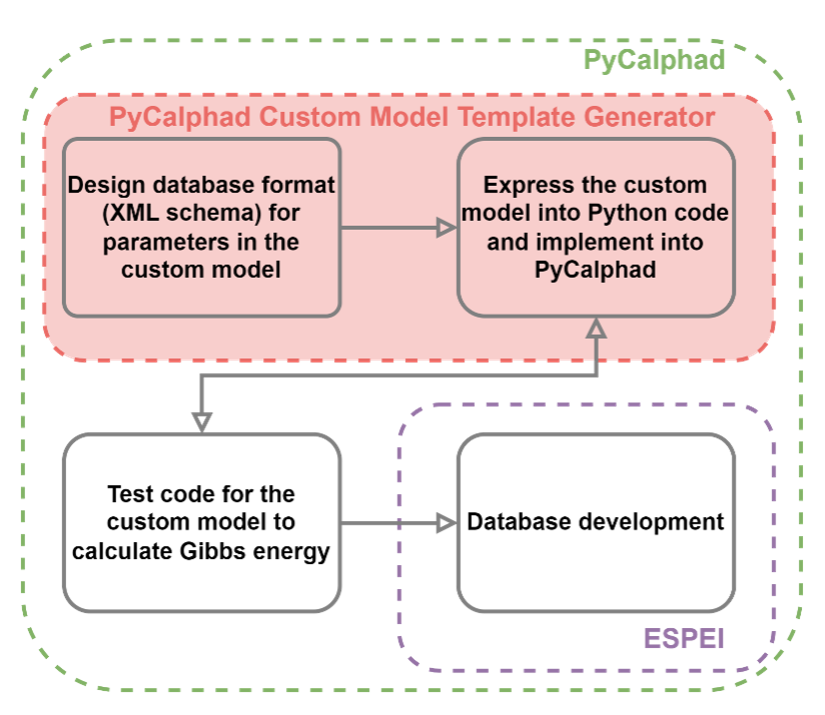
\includegraphics[width=0.75\linewidth]{models/Models-ImplementationFlow.png}
    \caption{Workflow for implementing custom models into PyCalphad and ESPEI.}
    \label{models:fig:implflow}
\end{figure}

\section{Implementation of UNIversal QUAsiChemical Model} \label{models:sec:UNIQUAC}
\subsection{UNIQUAC model} \label{models:ssec:UNIQUACfund}
The UNIQUAC model can be expressed using the CALPHAD nomenclature as follows:
\begin{equation} \label{models:eq:UQCGm}
    G_m=\sum_ix_i(^{o}G_i+RT\ln x_i) +\:^{cmb}G_m +\:^{res}G_m
\end{equation}
where $x_i$ is the mole fraction of constituent $i$, ${^o}G_i$ is the reference Gibbs energy of $i$, $\sum_ix_i^{o}G_i$ is considered as $^{srf}G_m$ term in (\ref{method:eq:Gm}). The second term $RT\sum_ix_i\ln x_i$ is configurational entropy contribution to Gibbs energy as $-T\:^{cnf}S_m$ term in (\ref{method:eq:Gm}). The excess Gibbs energy $^{xs}G_m$ are considered into two parts in the UNIQUAC, i.e., $^{cmb}G_m$ the combinatorial contribution of Gibbs energy and $^{res}G_m$ is the residual contribution of Gibbs energy.  

$^{cmb}G_m$ can be expressed as:
\begin{equation} \label{models:eq:UQCGcmb}
    ^{cmb}G_m=RT\sum_{i}{x_i\ln(\frac{\mathrm{\Phi}_i}{x_i}})+\frac{z}{2}\sum_{i}{x_iq_i\ln(\frac{\theta_i}{\mathrm{\Phi}_i}})
\end{equation}
\begin{equation} \label{models:eq:UQCphi}
    \mathrm{\Phi}_i=\frac{r_{i}x_i}{\sum_{j}{{r}_{j}x_j}}
\end{equation}
\begin{equation} \label{models:eq:UQCtheta}
    \theta_i= \frac{q_{i}x_i}{\sum_{j}{{q}_{j}x_j}}
\end{equation}
where $x_i$ is the mole fraction of constituent $i$, $r_i$ and $q_i$ are the component structural parameters, $r_i$ is the volume parameter, $q_i$ is the surface-area parameter, and $z$ is the average number of the nearest neighbors. $^{res}G_m$ can be expressed as:
\begin{equation} \label{models:eq:UQCres}
    {^{res}}G_m=-RT\sum_{i}{x_iq_i\ln(\rho_i})
\end{equation}
\begin{equation} \label{models:eq:rho}
    \rho_i=\sum_{j}{\theta_j\tau_{ji}}
\end{equation}
\begin{equation} \label{models:eq:UQCtau}
    \tau_{ji}=\exp \left(-\frac{u_{ij}-u_{ii}}{RT}\right)
\end{equation}
where $\Delta u_{ij}=u_{ij}-u_{ii}$ is the interaction parameter between $i$ and $j$, $u_{ii}$ represents the property of pure $i$. Thus, $\Delta u_{ij} \neq \Delta u_{ji}$ and $\tau_{ji} \neq \tau_{ij}$ Usually, $\Delta u_{ij}$ can be treated together as adjustable parameters during the modeling process.

%%%XML Database
To implement UNIQUAC into PyCalphad, a thermodynamic database containing the necessary parameters, such as $r_i$, $q_i$, and $\Delta u_{ij}$, is required. This database allows users to define these parameters, which PyCalphad can then read. To manage these newly defined parameters, an XML schema is employed as follows:
\begin{minted}[xleftmargin=1\parindent, linenos=true, fontsize=\small, breaklines=true]{xml}
<element name="Parameter">
    <attribute name="type">
        <choice>
            <value>UQCG</value><a:documentation>Gibbs energy of a specie</a:documentation>
            <value>UQCT</value><a:documentation>Tau function in residual contribution of excess Gibbs energy</a:documentation>
            <value>UQCQ</value><a:documentation>Surface-area parameter</a:documentation>
            <value>UQCR</value><a:documentation>Volume parameter</a:documentation>
            <value>UQCZ</value><a:documentation>Coordination number of a constituent</a:documentation>
        </choice>
    </attribute>
    <interleave>
        <optional>
            <text/>
        </optional>
        <zeroOrMore>
            <ref name="Interval"/>
        </zeroOrMore>
        <ref name="UNIQUACConstituentArray"/>
        <optional>
            <element name="Exponents">
                <list>
                    <data type="float"/>
                    <data type="float"/>
                </list>
            </element>
        </optional>
    </interleave>
</element>
\end{minted}
Here are the parts of the XML schema where parameters are defined. For example, by specifying \texttt{UQCQ}, the surface-area parameter $q_i$ can be defined. \texttt{UQCG} is the reference Gibbs energy ${^o}G_i$ in the (\ref{models:eq:UQCGm}), \texttt{UQCT} is the $\tau_{ji}$ function in residual contribution of excess Gibbs energy as shown in (\ref{models:eq:UQCtau}), \texttt{UQCR} is the volume parameter $r_i$, and \texttt{UQCZ} is the coordination number $z$.

The users now can adopt an XML thermodynamic database to input these parameters.
\begin{minted}[xleftmargin=1\parindent, linenos=true, fontsize=\small, breaklines=true]{xml}
<Parameter type='UQCQ'>1.72<ConstituentArray><Site refid="0"><Constituent refid="ACETONITRILE"/></Site></ConstituentArray></Parameter>
<Parameter type='UQCR'>1.87<ConstituentArray><Site refid="0"><Constituent refid="ACETONITRILE"/></Site></ConstituentArray></Parameter>
<Parameter type='UQCQ'>4.4<ConstituentArray><Site refid="0"><Constituent refid="N_HEPTANE"/></Site></ConstituentArray></Parameter>
<Parameter type='UQCR'>5.17<ConstituentArray><Site refid="0"><Constituent refid="N_HEPTANE"/></Site></ConstituentArray></Parameter>
<Parameter type="UQCZ">10<ConstituentArray><Site refid="0"><Constituent refid="ACETONITRILE"/></Site></ConstituentArray></Parameter>
<Parameter type="UQCZ">10<ConstituentArray><Site refid="0"><Constituent refid="N_HEPTANE"/></Site></ConstituentArray></Parameter>
<Parameter type="UQCT">exp(VV0001*T**(-1))<ConstituentArray><Site refid="0"><Constituent refid="ACETONITRILE"/><Constituent refid="N_HEPTANE"/></Site></ConstituentArray><Exponents>0.0 1.0</Exponents></Parameter>
<Parameter type="UQCT">exp(-545.71*T**(-1))<ConstituentArray><Site refid="0"><Constituent refid="ACETONITRILE"/><Constituent refid="N_HEPTANE"/></Site></ConstituentArray><Exponents>1.0 0.0</Exponents></Parameter>
\end{minted}

Here is an example of how to specify parameters for UNIQUAC in an XML thermodynamic database. First, define the type of parameter, such as \texttt{UQCQ}. Then, specify the value or function for that parameter. Following this, the name of the constituent can be defined using the \texttt{Constituent} tag.

\subsection{Calculations examples} \label{models:ssec:UNIQUACexamples}
With the implementation of the new UNIQUAC model in PyCalphad, users can automatically utilize all existing features in PyCalphad, including Gibbs energy minimization and phase diagram plotting. First, the calculation of Gibbs energy and its derivatives are carried out as a benchmark, comparing with calculation results from OpenCalphad \cite{li2020implementation}.

Figure \ref{models:fig:UQCGibbsE}, Figure \ref{models:fig:UQCS}, and Figure \ref{models:fig:UQCacr} depict the comparison between PyCalphad and OpenCalphad for calculating Gibbs energy, entropy, and activity, respectively. In PyCalphad, the \textit{calculate()} function was used to sample properties of a single phase, while the \textit{equilibrium()} function was utilized to perform global minimization of Gibbs energies and obtain phase equilibria. Both functions were thoroughly tested for UNIQUAC to ensure accurate calculations and minimization of Gibbs energy. The results demonstrate an excellent agreement between PyCalphad and OpenCalphad. 

affirming the successful implementation of UNIQUAC in PyCalphad.

\begin{figure}[H]
    \centering
    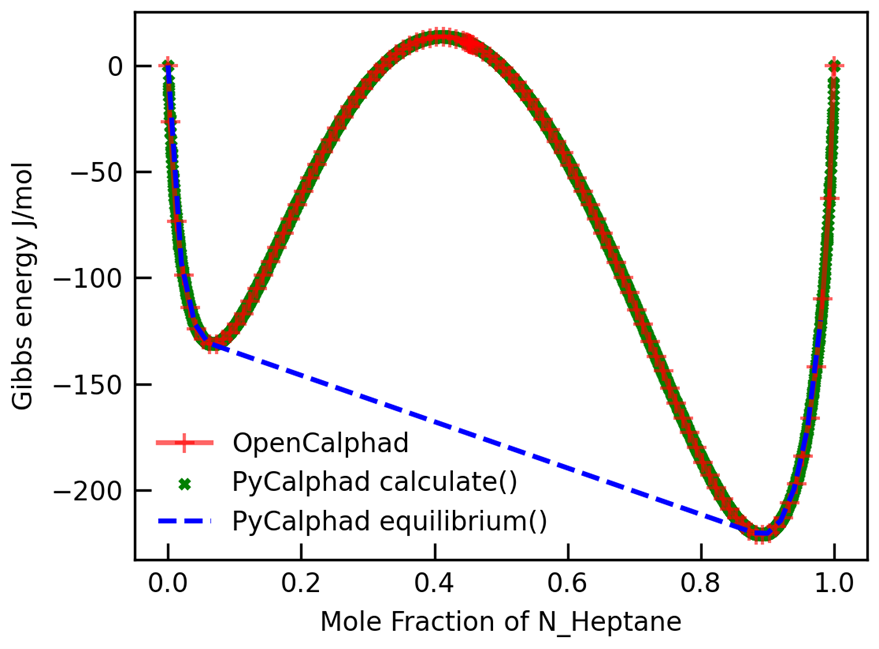
\includegraphics[width=0.5\linewidth]{models/Models-UQC-Gibbsenergy.png}
    \caption{Comparison of PyCalphad with OpenCalphad calculating Gibbs energy to verify the implementation of UNIQUAC. The red line represents results from OpenCalphad, the green $\times$ symbols represent results from the PyCalphad \textit{calculate()} function, and the blue line represents results from the PyCalphad \textit{equilibrium()} function.}
    \label{models:fig:UQCGibbsE}
\end{figure}

\begin{figure}[H]
    \centering
    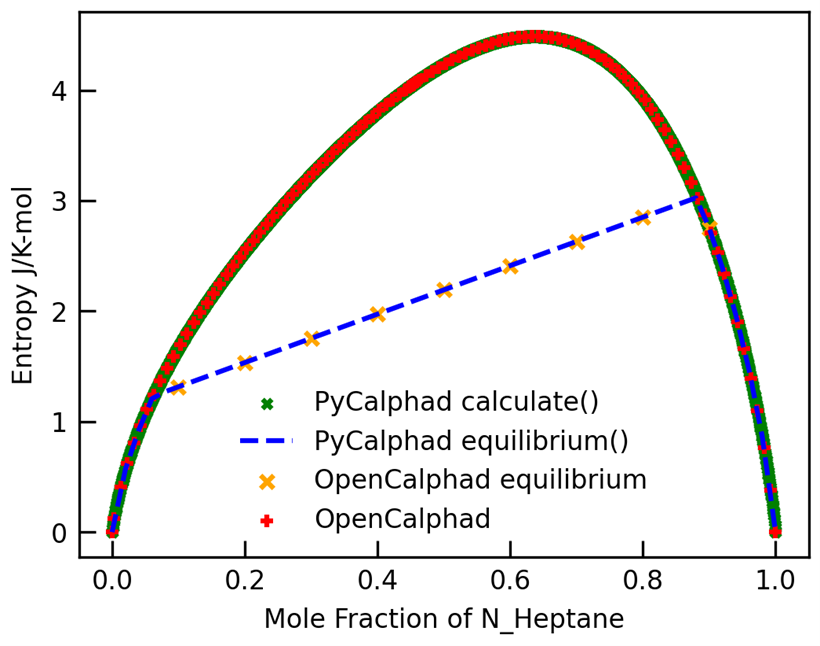
\includegraphics[width=0.5\linewidth]{models/Models-UQC-Entropy.png}
    \caption{Comparison of PyCalphad with OpenCalphad calculating entropy to verify the implementation of UNIQUAC. The red line represents results from OpenCalphad, the yellow $\times$ symbols represent results from OpenCalphad equilibrium calculations, the green $\times$ symbols represent results from the PyCalphad \textit{calculate()} function, and the blue line represents results from the PyCalphad \textit{equilibrium()} function.}
    \label{models:fig:UQCS}
\end{figure}

\begin{figure}[H]
    \centering
    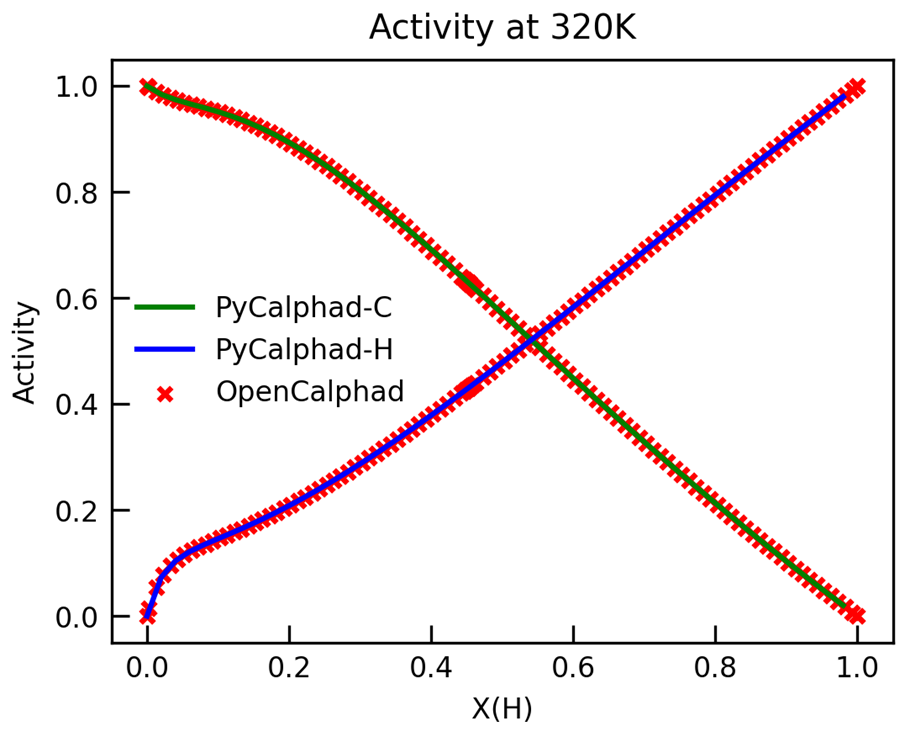
\includegraphics[width=0.5\linewidth]{models/Models-UQC-Activity.png}
    \caption{Comparison of PyCalphad with OpenCalphad calculating activity to verify the implementation of UNIQUAC. The red $\times$ symbols represent results from OpenCalphad; green and blue lines are calculated from PyCalphad.}
    \label{models:fig:UQCacr}
\end{figure}

Figure 4 and Figure 5 show the binary and ternary phase diagram for an artificial system modelled with UNIQUAC calculated from PyCalphad. The phase boundary matches well with phase diagram data obtained using OpenCalphad. These calculations and plots were generated using the existing functions in PyCalphad, namely \textit{equilibrium()} and \textit{eqplot()}. This alignment underscores the success of the UNIQUAC implementation in PyCalphad and demonstrates the robustness and capability of PyCalphad's existing functions for custom thermodynamic models.


\section{Custom model template generator} \label{models:sec:CMTG}


\subsection{Framework} \label{models:ssec:CMTGframework}


\subsection{Applications} \label{models:ssec:CMTGapp}


\section{Summary} \label{models:sec:Summary}
